\documentclass[10pt]{article}
\usepackage{pictex,amsmath,amsfonts,amssymb,amsthm,verbatim}
\usepackage{fullpage}
\usepackage{fullpage}
\usepackage{fancyhdr}
\usepackage{algorithm,algorithmic}
\usepackage{multirow}
\usepackage{gensymb}
\usepackage{mathrsfs}

\setlength{\voffset}{-0.25in}
\setlength{\headsep}{+0.5in}
\setlength{\parskip}{1em}
\setlength{\parindent}{0em}

\def\vu{\mathbf{u}}
\def\vv{\mathbf{v}}
\def\vb{\mathbf{b}}
\def\vw{\mathbf{w}}
\def\vs{\mathbf{s}}

\usepackage[lf]{Baskervaldx} % lining figures
\usepackage[bigdelims,vvarbb]{newtxmath} % math italic letters from Nimbus Roman
\usepackage[cal=boondoxo]{mathalfa} % mathcal from STIX, unslanted a bit
\renewcommand*\oldstylenums[1]{\textosf{#1}}
\usepackage{xcolor}
\usepackage{titlesec}
\usepackage{mdframed}
\usepackage[utf8]{vietnam}\newmdenv[linecolor=blue,skipabove=\topsep,skipbelow=\topsep,leftmargin=5pt,rightmargin=-5pt,innerleftmargin=5pt,innerrightmargin=5pt]{mybox}

\newcommand{\quotes}[1]{``#1''}
\usepackage{minted}
\usepackage{graphicx,graphics}

\begin{document}

\begin{center}
\huge Operating System
\end{center}

\section{Overview}

\quotes{What is Operating System ?}
\begin{itemize}
	\item An operating system acts an intermediary(trung gian) between the user of a computer and the computer hardware.
	\item Operating system provide an environment in which a user can execute programs in a \textit{convenient} and \textit{efficient} manner.
	\item An Operating System is software that manages the computer hardware, the hardware must provide appropriate mechanisms to ensure the correct operation and prevent user from interfering with the proper operation of the system.
\end{itemize}

\subsection{What Operating System can do ?}
\begin{enumerate}
	\item A computer system can be divided into 4 components: the \textbf{hardware}, the \textbf{operating system}, the \textbf{application programs}, and the \textbf{users}.
	\begin{itemize}
		\item The Hardware includes the \textbf{central unit processing} (CPU), the \textbf{memory}, and the \textbf{input-output} (IO) \textbf{devices}
		\item Hardware provides the basic computing resources for the system.
		\item The Application programs define the ways in which these resources are used to solve user's computing problem.
		\item The operating system controls the hardware and coordinates it use among the various application programs for various users.
		\item In system's view, the operating system is the program most intimately involved with the hardware. an operating system can be viewed as \textbf{resource allocator}.
		\item An operating system is a control program that manages the execution of user programs to prevent errors and improper use of the computer.
		\item An operating system is a program running at all times on the computer - usually called the \textbf{kernel}
	\end{itemize}

	\item \textbf{Computer-System Operation} 
	\begin{itemize}
		\item For a computer to start running, it needs to have an initial program to run or \textbf{bootstrap program}.
		\item Bootstrap program is stored in \textbf{ROM} (read-only memory) or \textbf{EEPROM} (electrically erasable programmable read-only memory) or \textbf{firmware}.
		\item Bootstrap program initializes all aspects of the system, it knows how to load the operating system and start executing that system.
		\item The operating system then starts executing the first process and waits for the occurrence events.
		\item The occurrence of an event is usually signaled by an \textbf{interrupt} from either software or hardware.

		\begin{itemize}
			\item Hardware may trigger an interrupt at any time by sending a signal to the CPU.
			\item Software may trigger a special operation called a \textbf{system call} or \textbf{monitor call}.
		\end{itemize}

	\end{itemize}

	\item \textbf{Interrupt: }
	\begin{itemize}
		\item When the CPU is interrupted, it stops what it is doing and immediately transfers execution to a fixed location.
		\item The fixed location usually contains the starting address where service routine for the interrupt is located.
		\item The interrupt must transfer control to the appropriate interrupt service routine.
		\item The \textbf{interrupt vector} provide the address of the interrupt service routine for the interrupting device.
		\item The interrupt architecture must also save the address of the interrupted instruction.
		\item Incoming interrupts are disabled while another interrupt is being processed to prevent a \textbf{lost interrupt}
		\item A \textbf{trap} is a software-generated interrupt caused either by an error or a user request.
		\item An operating system is \textbf{interrupt driven}. 
	\end{itemize}

	\item \textbf{Storage Structure}
	\begin{itemize}
		\item General-purpose computers run most of their program from rewritable memory, called main memory (or random-access memory (RAM)).
		\item Main memory is commonly implemented in a semiconductor technology called \textbf{dynamic random-access memory} (DRAM).
		\item Main memory is usually too small to store all needed programs and data permanently.
		\item Main memory is a \textit{volatile} storage device that loses its contents when power is turned off or otherwise lost.
		$\rightarrow$ \textbf{secondary storage} for larges quantities of data permanently.
		\item \textbf{magnetic disk}: provide storage for both program and data.
		\item Most programs (system and application) are storage on a disk until they are loaded into memory.
		\item Differences between among the various storage systems lie on speed, cost, size and volatility.

		\bigbreak
		%\includegraphics[scale = 0.3]{hinh.png}
		\bigbreak

		\item In the absence of power and general backup systems, some data must be written to \textbf{nonvolatile storage}.
		\item Some nonvolatile disks are electronic disk, NVRAM (DRAM with battery backup power).
	\end{itemize}

\end{enumerate}

\pagebreak
\section*{Chapter 3: Process}

\subsection*{Process Concept}
\begin{enumerate}
	\item \textbf{The Process}
	\begin{itemize}
		\item The process:
		\begin{itemize}
			\item A process is a program in execution.
			\item The status of the current activity of a process is represented by the value of the \textbf{program counter} and the contents of the processor's register. 
			\item The memory layout of a process is typically divided into multiple sections
			\begin{itemize}
				\item \textbf{Text section:} - the executable code 
				\item \textbf{Data section:} - global variables
				\item \textbf{Heap section:} - memory that is dynamically allocated duirng program run time.
				\item \textbf{Stack section:} - temporary data storage when invoking functions (parameters, return val, ... etc).
				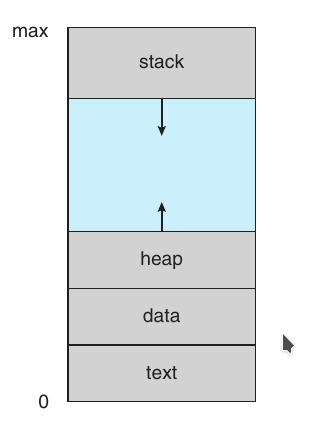
\includegraphics[width=5cm]{memory_layout.png}
				\bigbreak
			\end{itemize}

			\item The size of text and data section is \textbf{fixed}, while the stack and heap section can shrink and grow \textbf{dynamically} during program execution.
			\item the stack and heap sections grow \textbf{toward} one another, the operating system must ensure they do not \textbf{overlap} one another.
			\item A program itself is not a process, which is called \textbf{passive entity} while process is called \textbf{active} entity with a program counter specifying the next instruction to execute and a set of associated resources.
			\item A program become a process when when an executable file is loaded into a memory.
			\item Two processes may be associated with the same program, they are nevertheless considered two separate execution sequences.
			\item A process can itself be an execution environment for another code. For instance, the JVM   
		\end{itemize}
	\end{itemize}

	\item \textbf{Process State}
	\begin{itemize}
		\item The state of the process is defined in part of the current activity of that process.
		\begin{itemize}
			\item \textbf{New}: The process is being created.
			\item \textbf{Running}: Instructions are being executed.
			\item \textbf{Waiting}: The process is waiting for some events to occur (such as I/O completion or reception of a signal).
			\item \textbf{Ready}: The process is waiting to be assigned to a processor.
			\item \textbf{Terminated}: The process has finished execution.
		\end{itemize}

		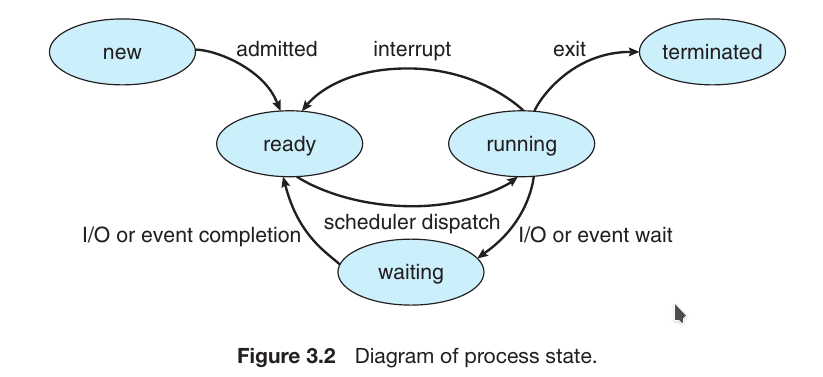
\includegraphics[scale=0.6]{Process_state.png}
		\\
		\bigbreak

		\item Only \textbf{one} process can be \textit{running} on any processor core at any instant. Many process may be \textit{ready} and \textit{waiting}. 
	\end{itemize}

	\item \textbf{Process Control Block}
	\begin{itemize}
		\item Each process is represented in the operating system by a \textbf{process control block (PCB)} or \textbf{task control block}.
		\begin{itemize}
			\item Process state
			\item Program counter
			\item CPU register
			\item CPU-scheduling information
			\item Memory-management information
			\item Accounting information
			\item I/O status information
		\end{itemize}
	\end{itemize}

	\item \textbf{Threads}
	\begin{itemize}
		\item A process is a program that performs a single \textbf{thread} of execution.
	\end{itemize}
\end{enumerate}

\subsection*{Process Scheduling}

\begin{itemize}
	\item The objective of multiprogramming is to have some process running at all the times so as to maximize CPU utilization.
	\item The objective for time sharing is to switch a CPU core among processes so frequently that users can interact with each program while it is running.
	\item To meet those objective, \textbf{process scheduler} is used to select an available process for program execution on a core.
	\item The number of processes currently in memory is known as the \textbf{degree of multiprogramming}.
	\item Most processes can be described as either I/O bound or CPU bound.
	\begin{itemize}
		\item An \textbf{I/O bound process} is one that spends more of its time doing I/O than it spends doing computations.
		\item A \textbf{CPU-bound process} generates I/O requests infrequently, using more of its time doing computations. 
	\end{itemize}
\end{itemize}

\begin{enumerate}
	\item \textbf{Scheduling Queues}
	\begin{itemize}
		\item As a processes enter the system, they are put into the \textbf{ready queue}, where they are ready and waiting to execute on a CPU's core. This queue is a linked-list.
		\item When a process is allocated a CPU core, it executes for a while and eventually terminates, is interrupted, or waits for the occurrence of a particulat event - I/O request. Therefore, the process has to wait for the completion of I/O - which is placed in a \textbf{wait queue}. 
	\end{itemize}

	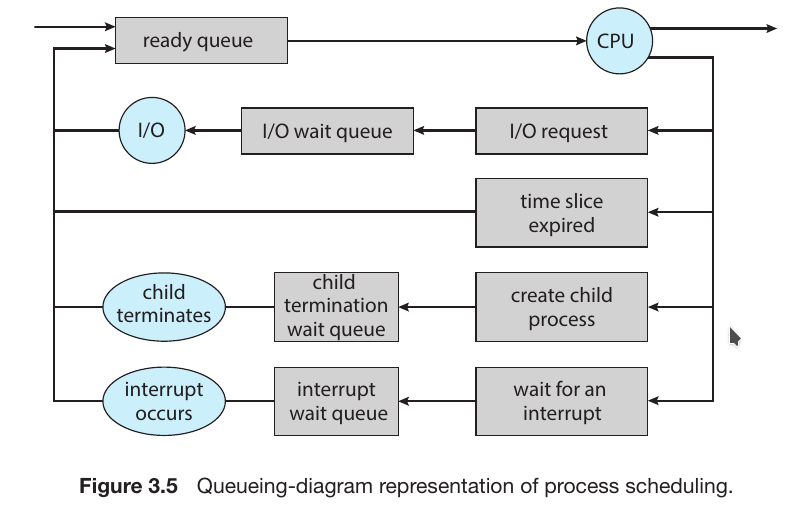
\includegraphics[scale=0.6]{Queueing-diagram.png}
	\\
	\bigbreak

	\item \textbf{CPU Scheduling}
	\begin{itemize}
		\item The role of \textbf{CPU scheduler} is to select from among the processes that are in the ready queue and allocate a CPU core to one of them.
		\item The scheduler must select a new process for the CPU frequently.
	\end{itemize}
\end{enumerate}

\end{document}